\section{Theory - Vortex Methods}
\subsection{Introduction}
This section serves to out line how Vortex Methods work, it provides a description however it does not a strict proof. The simulation will be split into two parts, the convective scheme and the discretization scheme, this puts into context the subsequent two theory sections which examine each scheme in greater detail. The description given here is provided for a 2D flow, the vortex method developed in this report is 3D however only a 2D description is provided for brevity.
\subsection{Theory}
The Navier-Stokes equations are a set of equations that govern fluid flow assuming continuum conditions apply. The Navier-Stokes are equations are shown in equations \ref{eq:NS1} through to \ref{eq:NS3}. Equation \ref{eq:NS1} is the continuity equation and enforces the incompressibility and conservation off mass of the fluid. Equation \ref{eq:NS2} is the momentum equation and describes the evolution of the fluid velocity ensuring the conservation of linear momentum. Equation \ref{eq:NS3} is the energy equation and describes the evolution of fluid temperature. These equations are often solved by either an iterative method or simplifications are introduced so an analytical solution can be used.

\begin{equation}
\label{eq:NS1}
div(\vec{V})=0
\end{equation}

\begin{equation}
\label{eq:NS2}
\frac{\partial V}{\partial t}+V\cdot\nabla V-\nu\nabla^2 V+\frac{1}{\rho} \nabla P=F
\end{equation}

\begin{equation}
\label{eq:NS3}
\frac{\partial T}{\partial t}+V\cdot T -\alpha \nabla^2 T=\frac{s}{\rho c}
\end{equation}

For the simulation discussed here a number of assumptions are made. Firstly the fluid is incompressible, this automatically satisfies equation \ref{eq:NS1} and secondly the fluid is isentropic with constant thermo-physical properties, this automatically satisfies equation \ref{eq:NS3}. This leaves us with only equation \ref{eq:NS2}, the momentum equation, to consider.

\begin{equation}
\label{eq:momen1}
\frac{\partial V_X}{\partial t}+v_X \frac{\partial V_X}{\partial x}+V_Y \frac{\partial V_X}{\partial y}-\nu\big(\frac{\partial^2 V_X}{\partial x^2}+\frac{\partial^2 V_Y}{\partial y^2}\big)+\frac{1}{\rho}\frac{\partial P}{\partial x}=F_X
\end{equation}

\begin{equation}
\label{eq:momen2}
\frac{\partial V_y}{\partial t}+v_X \frac{\partial V_y}{\partial x}+V_Y \frac{\partial V_y}{\partial y}-\nu\big(\frac{\partial^2 V_y}{\partial x^2}+\frac{\partial^2 V_y}{\partial y^2}\big)+\frac{1}{\rho}\frac{\partial P}{\partial y}=F_y
\end{equation}

Equations \ref{eq:momen1} and \ref{eq:momen2} represent the momentum equation in Cartesian coordinates for a 2D flow. These two equations are non-linear PDE's and have no analytical solution. To simplify them further it is assumed that the flow is inviscid and the only external force acting upon it is gravity in addition to being isentropic and incompressible. This results in equations \ref{eq:momen3} and \ref{eq:momen4}

\begin{equation}
\label{eq:momen3}
\frac{\partial V_x}{\partial t}+v_x \frac{\partial V_x}{\partial x}+V_y \frac{\partial V_x}{\partial y}+\frac{1}{\rho}\frac{\partial P}{\partial x}=g_x
\end{equation}

\begin{equation}
\label{eq:momen4}
\frac{\partial V_y}{\partial t}+v_x \frac{\partial V_y}{\partial x}+V_y \frac{\partial V_y}{\partial y}+\frac{1}{\rho}\frac{\partial P}{\partial y}=g_y
\end{equation}

Equations \ref{eq:momen3} and \ref{eq:momen4} represent the momentum equation and describes the evolution of the velocity of the fluid in Cartesian coordinates. In order to describe the evolution of the fluid in terms of vorticity the curl of the momentum equation is taken, in Cartesian coordinates this is performed via equation \ref{eq:CurlDef}. The vorticity of a flow is defined as the curl of the velocity vector, for a 2D flow this is given by equation \ref{eq:VortDef} and is simply equation \ref{eq:CurlDef} applied to a velocity vector with only i and j components.

\begin{equation}
\label{eq:CurlDef}
curl(\vec{F})=\big(\frac{\partial F_z}{\partial zy}-\frac{\partial F_y}{\partial z}\big)\hat{i}+\big(\frac{\partial F_x}{\partial z}-\frac{\partial F_z}{\partial x}\big)\hat{j}+\big(\frac{\partial F_y}{\partial x}-\frac{\partial F_x}{\partial y}\big)\hat{k}
\end{equation}

\begin{equation}
\label{eq:VortDef}
\omega=\Big(\frac{\partial V_y}{\partial x}-\frac{\partial V_x}{\partial y}\Big)
\end{equation}

In equation \ref{eq:CurlDef} the function $\vec{F}$ represents the momentum equation. For a 2D flow the vorticity vector has only one component perpendicular to the flow plane, hence for our momentum equation the definition for curl is calculated by equation \ref{eq:MomenCurl}

\begin{equation}
\label{eq:MomenCurl}
curl(\vec{F})=\big(\frac{\partial F_y}{\partial x}-\frac{\partial F_x}{\partial y}\big)\hat{k}
\end{equation}

Hence to calculate the the curl of the momentum equation we need to calculate the partial derivatives of equations \ref{eq:momen3} and \ref{eq:momen4} with respect to the y and x directions respectively. This is shown in equations

\begin{equation}
\label{eq:DerivX}
\frac{\partial F_x}{\partial y} = \frac{\partial}{\partial y}\Big(\frac{\partial V_x}{\partial t}+v_x \frac{\partial V_x}{\partial x}+V_y \frac{\partial V_x}{\partial y}+\frac{1}{\rho}\frac{\partial P}{\partial x}\Big)
\end{equation}

\begin{equation}
\label{eq:DerivY}
\frac{\partial F_y}{\partial x} = \frac{\partial}{\partial x}\Big(\frac{\partial V_y}{\partial t}+v_x \frac{\partial V_y}{\partial x}+V_y \frac{\partial V_y}{\partial y}+\frac{1}{\rho}\frac{\partial P}{\partial y}\Big)
\end{equation}

Equations \ref{eq:DerivX} and \ref{eq:DerivY} are first simplified by assuming the pressure variation in the wake is sufficiently small so that in can be neglected, this is not a practical assumption for air traveling over the aerofoil, however it is applicable to the wake region to be modelled. This reduces equations \ref{eq:DerivX} and \ref{eq:DerivY} to equations \ref{eq:DerivX2} and \ref{eq:DerivY2} respectively.

\begin{equation}
\label{eq:DerivX2}
\frac{\partial F_x}{\partial y} = \frac{\partial}{\partial y}\Big(\frac{\partial V_x}{\partial t}+v_x \frac{\partial V_x}{\partial x}+V_y \frac{\partial V_x}{\partial y}\Big)
\end{equation}

\begin{equation}
\label{eq:DerivY2}
\frac{\partial F_y}{\partial x} = \frac{\partial}{\partial x}\Big(\frac{\partial V_y}{\partial t}+v_x \frac{\partial V_y}{\partial x}+V_y \frac{\partial V_y}{\partial y}\Big)
\end{equation}

Performing the differentiations in equations \ref{eq:DerivX2} and \ref{eq:DerivY2} yields

\begin{equation}
\label{eq:DerivX3}
\frac{\partial F_x}{\partial y}=\frac{\partial}{\partial y}\frac{\partial V_x}{\partial t}+\frac{\partial V_x}{\partial y}\frac{\partial V_x}{\partial x}+V_x\frac{\partial}{\partial y}\frac{\partial V_x}{\partial x}+\frac{\partial V_y}{\partial y}\frac{\partial V_x}{\partial y}+V_y\frac{\partial}{\partial y}\frac{\partial V_x}{\partial y}
\end{equation}

\begin{equation}
\label{eq:DerivY3}
\frac{\partial F_y}{\partial x}=\frac{\partial}{\partial x}\frac{\partial V_y}{\partial t}+\frac{\partial V_x}{\partial x}\frac{\partial V_y}{\partial x}+v_x\frac{\partial}{\partial x}\frac{\partial V_y}{\partial x}+\frac{\partial V_y}{\partial  x}\frac{\partial V_y}{\partial y}+V_y\frac{\partial}{\partial x}\frac{\partial V_y}{\partial y}
\end{equation}

Substituting equations \ref{eq:DerivX3} and \ref{eq:DerivY3} into equation \ref{eq:MomenCurl} and factorising then yields equation \ref{eq:Helmholtz1}. The equation is equal to $0$ as the right hand sides of equations \ref{eq:momen3} and \ref{eq:momen4} are gravitational constant that go to zero when differentiated.


\begin{equation}
\label{eq:Helmholtz1}
\frac{\partial}{\partial t}\Big(\frac{\partial V_y}{\partial x}-\frac{\partial V_x}{\partial y}\Big)+V_x\frac{\partial}{\partial x}\Big(\frac{\partial V_y}{\partial x}-\frac{\partial V_x}{\partial y}\Big)+V_y\frac{\partial}{\partial y}\Big(\frac{\partial V_y}{\partial x}-\frac{\partial V_x}{\partial y}\Big)+\Big(\frac{\partial V_x}{\partial x}+\frac{\partial V_y}{\partial y}\Big)\Big(\frac{\partial V_y}{\partial x}-\frac{\partial V_x}{\partial y}\Big)=0
\end{equation}

In equation \ref{eq:Helmholtz1} there is a common factor throughout all terms, this is the aforementioned definition for vorticity given in \ref{eq:VortDef}. Substituting equation \ref{eq:VortDef} into equation \ref{eq:Helmholtz1} yields equation \ref{eq:Helmholtz2}

\begin{equation}
\label{eq:Helmholtz2}
\frac{\partial \omega}{\partial t}+V_x\frac{\partial \omega}{\partial x}+V_y\frac{\partial \omega}{\partial y}+\omega \Big(\frac{\partial V_x}{\partial x}+\frac{\partial V_y}{\partial y}\Big)=0
\end{equation}

In the last term in equation \ref{eq:Helmholtz2} the vorticity is multiplied by two partial differentials. This term is the divergence of the velocity, we previously defined the fluid to be incompressible, hence according to equation \ref{eq:NS1} this term is zero. Hence equation \ref{eq:Helmholtz2} becomes \ref{eq:Helmholtz3}

\begin{equation}
\label{eq:Helmholtz3}
\frac{\partial \omega}{\partial t}+V_x\frac{\partial \omega}{\partial x}+V_y\frac{\partial \omega}{\partial y}=0
\end{equation}

Equation \ref{eq:Helmholtz3} is a form of the vorticity equation for a 2D inviscid incompressible flow in a Eulerian reference frame, it describes the evolution of vorticity with respect to time. In order to use this for a Lagrangian simulation this equation needs to be written in terms of a Largrangian reference frame. A definition for the material Derivative is given in equation \ref{eq:MaterialDerv} for a arbitrary variable $\varphi$ traveling in a fluid of velocity $\vec{V}$

\begin{equation}
\label{eq:MaterialDerv}
\frac{D(\varphi)}{Dt}=\frac{\partial (\varphi)}{\partial t}+\vec{V}\nabla \varphi
\end{equation}

Hence substituting $\varphi$ for $\omega$ and expansing yields equation \ref{eq:HelmHoltz4}

\begin{equation}
\label{eq:HelmHoltz4}
\frac{D\omega}{Dt}=\frac{\partial \omega}{\partial t}+V_x\frac{\partial \omega}{\partial x}+V_y\frac{\partial \omega}{\partial y}
\end{equation}

Substituting the results of equation \ref{eq:Helmholtz3} into equation \ref{eq:HelmHoltz4} results in equation \ref{eq:Helmholtz5}

\begin{equation}
\label{eq:Helmholtz5}
\frac{D\omega}{Dt}=0
\end{equation}

Equation \ref{eq:Helmholtz5} represents Helmholtz's equation. The result of this equation is significant, it governs the evolution of vorticity of a fluid in a Lagrangian reference frame. However, as can be seen, there is no change in vorticity with respect to time, the vorticity is constant. Hence, a packet of fluid evolving with time and translating has constant vorticity. For a particle based simulation this means that all particles conserve their vorticity.
\\\\
Hence we know the vorticity of a series of particles of fluid at any point in time, however to determine their position the velocity field needs to be determined. The velocity field is recovered from the vorticity through the Biot-Savart law, shown in equation \ref{eq:BiotSavart}

\begin{equation}
\label{eq:BiotSavart}
\vec{V}(x,y,z)=\frac{\Gamma}{4\pi}\int_{+\infty}^{-\infty} \frac{d\vec{\ell}\times\vec{r}}{|\vec{r}|^3}
\end{equation}

The Biot-Savart law allows for the calculation of the induced velocity at any point due to a vortex filament hence the integral across a length (extending to infinity if the fluid has no boundaries due to Helmholtz's second theorem). However in the present simulation continuous vortex filaments are approximated to a series of discrete points.

\begin{figure}[H]
\centering
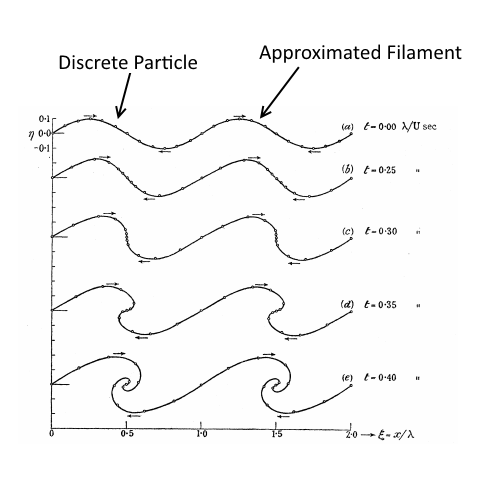
\includegraphics[width=0.8\textwidth]{Referenced_Figures/RosenheadApproximation.png}
\caption{\label{fig:RosenheadFig} $ON^2$ Increase in Complexity Demonstrated for an Unoptimized Case}
\end{figure} 

Figure \ref{fig:RosenheadFig} is taken from Rosenhead's original paper and shows a series of discrete vortex particles (the larger dots along the lines) approximating a vortex filament (\cite{rosenhead_1931}). The filament is drawn as an interpolating function along the discrete points. The figure also shows Rosenhead's original simulation with every filament drawn being the evolution after a certain time of the filament above it. 
\\\\
The Biot-Savart law given in equation \ref{eq:BiotSavart} assumed a velocity field induced by a vortex filament, if discrete vortex points are used then the equation reduces to equation \ref{eq:BiotSavart2}

\begin{equation}
\label{eq:BiotSavart2}
\vec{V}(x,y,z)=\frac{\Gamma \times \vec{r}}{4\pi \times |\vec{r}|^3} 
\end{equation}

Equation \ref{eq:BiotSavart2} gives the velocity field induced by a single discrete vortex. The velocity induced by a series of discrete vortex particles is the superposition of the velocity fields induced by every individual element. Given a number $N$ of elements, the velocity field at any point is given by equation 

\begin{equation}
\label{eq:BiotSavart3}
\vec{V}(x,y,z)=\sum_{i=0}^{N}\frac{\Gamma_i \times \vec{r_i}}{4\pi \times |\vec{r_i}|^3} 
\end{equation}

Hence a full description of the flow field is obtained. The particles have a initial vorticities, which stay constant throughout the simulation. Their velocities can be extracted from their initial positions and vorticities. Using the velocity field their positions can be incremented for a finite time period $\delta t$ and the process repeated

\subsection{Simulation Algorithm}

Figure \ref{fig:Algorithm} shows the basic algorithm implemented for any vortex method. The algorithm starts by with the definition of the initial conditions of the simulation. The velocity field is then calculated via the Biot-Savart law, this is knows as the "Convective Scheme". The positions of the elements are then iterated over a finite time step $\delta t$, this is known as the "Discretization Scheme". The output is then displayed to the user via the "Rendering Scheme". Both the "Convective Scheme" and the "Discretization" scheme are discussed in further detail in their respective theory sections. The "Rendering Scheme" is not discussed however the code is included in the appendix.

\begin{figure}[H]
\centering
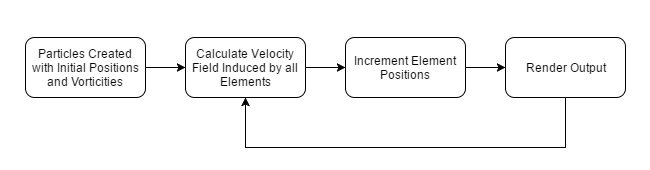
\includegraphics[width=1.0\textwidth]{Figures/Algorithm.png}
\caption{\label{fig:Algorithm} Eulers method used to approximate $f(x)=e^x-1$ for 5 different time steps}
\end{figure} 







